\documentclass[%
pdf,
%nocolorBG,
colorBG,
slideColor,
tcrico,
%slideBW,
%draft,
%frames
%azure
%contemporain
%nuancegris
%troispoints
%lignesbleues
%darkblue
%alienglow
%autumn
%default
%gyom
%blends
]{prosper}
\usepackage{amsmath}
%\usepackage[table]{xcolor}
\usepackage{colortbl}
\usepackage{graphicx}
\usepackage{algorithm2e}

\begin{document}

\begin{slide}{Knowledge Based Technologies}
\large
\textbf{Lecture 2} 
\newline
\textbf{Induction Learning}

\bigskip
\small
John Moore \& Thomas Collins



\end{slide}

%%%%%%%%%%%%%%%%%%%%%%%%%%%%%%%%


\begin{slide}{Lecture Overview}
\begin{itemize}
\item Learning from examples
\item General-to-specific ordering over hypotheses
\item Version spaces and candidate elimination algorithm
\item Picking new examples
\item The need for inductive bias
\end{itemize}
\end{slide}

%%%%%%%%%%%%%%%%%%%%%%%%%%%%%%%%


\begin{slide}{An Example}
	\begin{center}
	\tiny
	\begin{tabular}{ccccccc} \hline
	\rowcolor[HTML]{99aabb}\textbf{Sky} & \textbf{Temp} & \textbf{Humid} & \textbf{Wind} & \textbf{Water} & \textbf{Forecast}& \textbf{Play Sport}
	\\ \hline \hline
	\rowcolor[HTML]{bbccdd} Sunny   & Warm    & Normal & Strong  & Warm    & Same      & Yes \\
	\rowcolor[HTML]{ccddee}Sunny   & Warm    & High   & Strong  & Warm    & Same      & Yes \\
	\rowcolor[HTML]{bbccdd} Rainy    & Cold    & High   & Strong  & Warm    & Change     & No \\
	\rowcolor[HTML]{ccddee}Sunny    & Warm    & High   & Strong  & Cool    & Change    & Yes \\ 
	\end{tabular}
	\end{center}
\begin{itemize}
\item What is the general concept?
\end{itemize} 

\end{slide}

%%%%%%%%%%%%%%%%%%%%%%%%%%%%%%%%



\begin{slide}{Representing Hypotheses}
\begin{itemize}
\item Many possible representations
\item Here the hypothesis is conjunction of constraints on attributes
\item Each constraint can be
	\begin{itemize}
	\item a specific value (e.g., $Water=Warm$)
	\item don't care (e.g., ``$Water=?$'')
	\item no value allowed (e.g.,``Water=$\emptyset$'') 
	\end{itemize}
\item For example,
	\tiny
	\begin{tabular}{ccccccc} 
	\rowcolor[HTML]{bbccdd} Sky & AirTemp & Humid & Wind & Water & Forecast 
 	\\ \hline \hline
	\rowcolor[HTML]{bbccdd} $\langle Sunny$   & $?$    & $?$ & $Strong$  & $?$    & $Same \rangle$
	\end{tabular}
\end{itemize}
\end{slide}

%%%%%%%%%%%%%%%%%%%%%%%%%%%%%%%%


\begin{slide}{Prototypical Concept Learning Task}
\tiny
\begin{itemize}
 \item  {\bf Given:} 
	\begin{itemize}
	\item Instances $X$: Possible days, each described by the attributes {\em Sky, AirTemp, Humidity, Wind, Water, Forecast}
	\item Target function $c$: $EnjoySport: X \rightarrow \{0,1 \}$
	\item Hypotheses $H$: Conjunctions of literals. E.g. \[\langle ?, Cold, High, ?, ?, ? \rangle. \]
	\item Training examples $D$: Positive and negative examples of the target function \[\langle x_1, c(x_1) \rangle , \ldots \langle x_m, c(x_m) \rangle\]
	\end{itemize}
\item {\bf Determine:}
A hypothesis $h$ in $H$ such that $h(x)=c(x)$ for all $x$ in $D$.
%\begin{itemize}
%\item[] ?
%A hypothesis $h$ in $H$ such that $h(x)=c(x)$ for all $x$ in $X$.
%
%\item
%(A hypothesis $h$ in $H$ such that $h(x)=c(x)$ for all $x$ in $D$.)
%\end{itemize}
\end{itemize}

\end{slide}

%%%%%%%%%%%%%%%%%%%%%%%%%%%%%%%%



\begin{slide}{The Inductive Learning Hypothesis}
\begin{itemize}
\item Any hypothesis found to approximate
the target function well over a sufficiently large set of training examples
will also approximate the target function well over other unobserved examples.
\end{itemize}
\end{slide}

%%%%%%%%%%%%%%%%%%%%%%%%%%%%%%%%
\begin{slide}{Hypothesis Space Ordering}
\begin{figure}
	\centering
	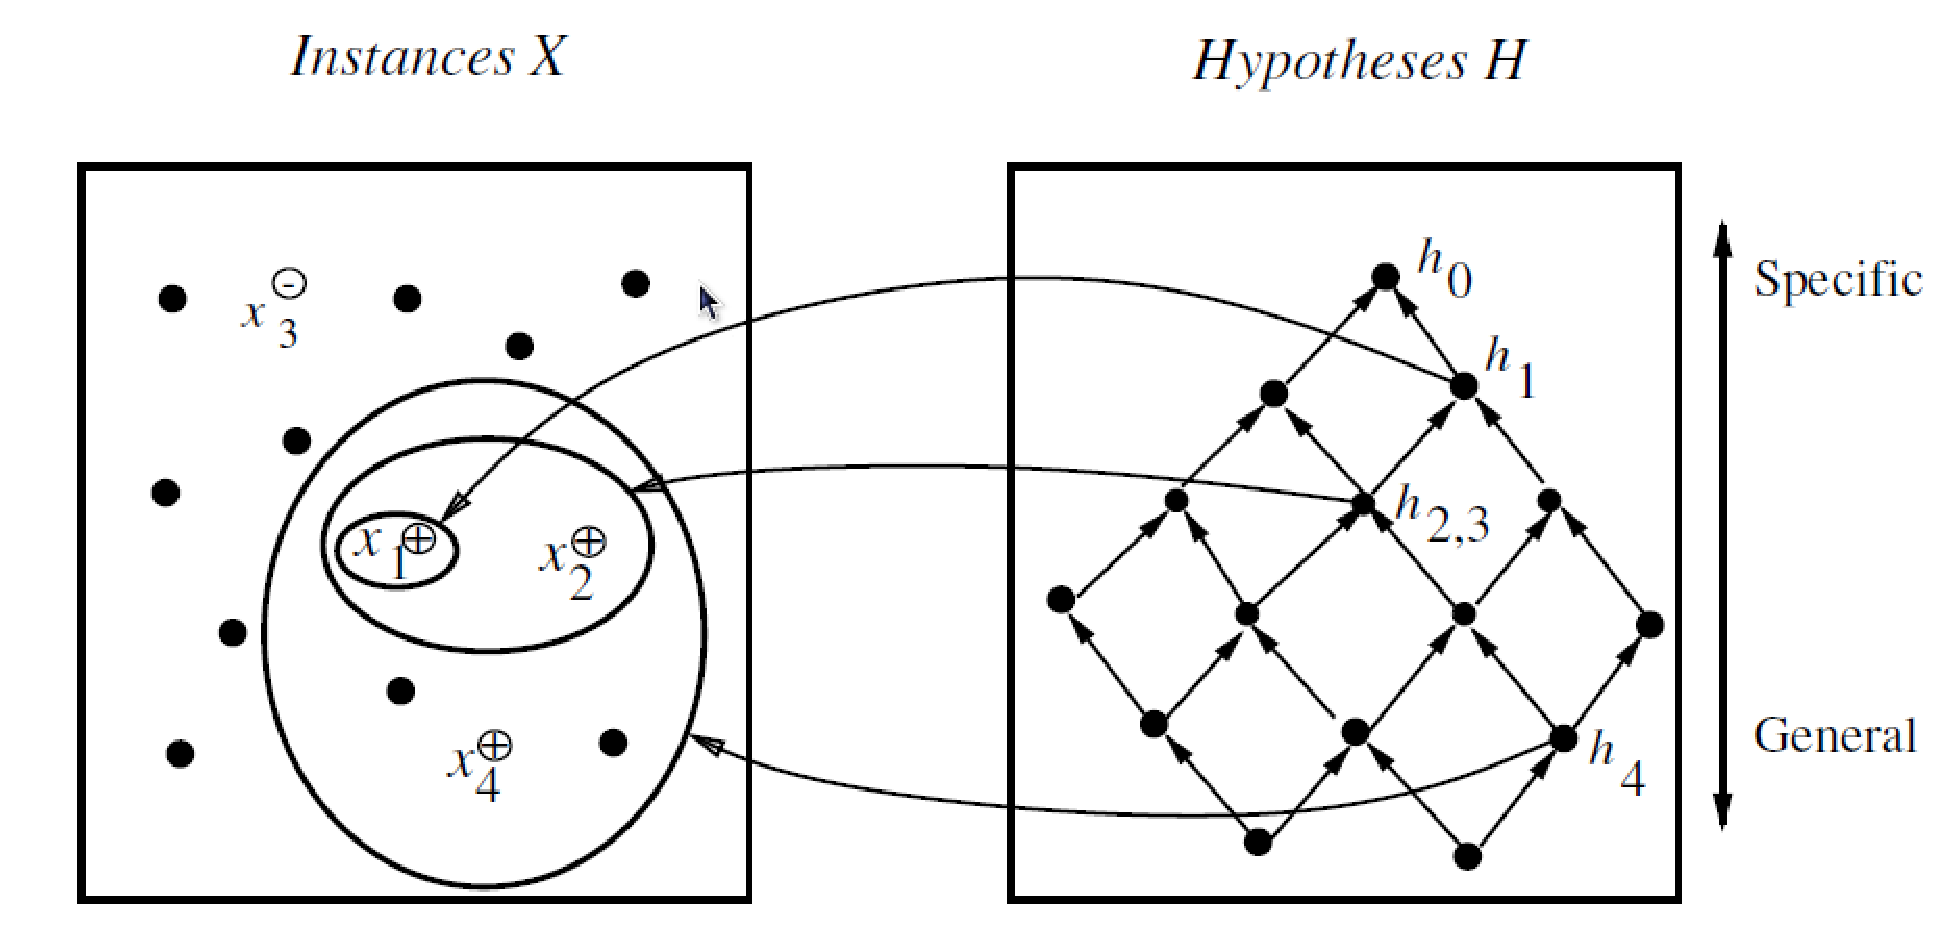
\includegraphics[scale=0.3]{hypoSpace.eps}
\end{figure}
\end{slide}

%%%%%%%%%%%%%%%%%%%%%%%%%%%%%%%%
\begin{slide}{Hypothesis Space Ordering ctd..}
\tiny
\begin{itemize}
\item The first box represents the set of all instances X. Each point is an instance. 
\item The circles are hypothesis. The points inside a circle correspond to the instances that hypothesis classifies as positive.
	\begin{itemize}
	\item $x_1 =\{Sunny,Warm,High,Strong,Cool,Same\}$
	\item $x_2 = \{Sunny,Warm,High,Light,Warm,Same\}$
	\end{itemize}
\item The second box represents an ordered set of all the possible hypothesis. 
\item The ones higher up are more specific, the lower more general.
\item The top will contain the hypothesis that classifies all	examples as negative while the bottom with the hypothesis that classifies every example as positive.
	\begin{itemize}	
	\item $h_1 =\{Sunny,?,?,Strong,?,?\}$
	\item $h_2 =\{Sunny,?,?,?,?,?\}$
	\item $h_3 = \{Sunny,?,?,?,Cool,?\}$
	\end{itemize}
\end{itemize}
\end{slide}

%%%%%%%%%%%%%%%%%%%%%%%%%%%%%%%%


\begin{slide}{The Find S Algorithm}

\begin{enumerate}
\item Initialize $h$ to the most specific hypothesis in $H$
\item For each positive training instance $x$
	\begin{itemize}
	\item For each attribute constraint $a_{i}$ in $h$
		\begin{itemize}
		\item If the constraint $a_{i}$ in $h$ is satisfied by $x$ Then do nothing
		\item Else replace $a_{i}$ in $h$ by the next more general constraint that is satisfied by $x$
		\end{itemize}
	\end{itemize}
\item Output hypothesis $h$
\end{enumerate}
\end{slide}

%%%%%%%%%%%%%%%%%%%%%%%%%%%%%%%%

\begin{slide}{Find S Algorithm Hypothesis Space Search}
\begin{figure}
	\centering
	\includegraphics[scale=1.0]{../bookps/finds-gen-spec.ps}
\end{figure}
\end{slide}

%%%%%%%%%%%%%%%%%%%%%%%%%%%%%%%%


\begin{slide}{Issues with Find S }
\begin{itemize}
 	\item Can't tell whether it has learned concept
	\item Can't tell when training data inconsistent
	\item Picks a maximally specific $h$ (why?)
	\item Depending on $H$, there might be several!
\end{itemize}
\end{slide}

%%%%%%%%%%%%%%%%%%%%%%%%%%%%%%%%

\begin{slide}{Version Spaces}
\begin{itemize}
 	\item  A hypothesis $h$ is {\bf consistent} with a set of training examples $D$ of
target concept $c$ if and only if $h(x)=c(x)$ for each training example
$\langle x, c(x) \rangle$ in $D$.
\[Consistent(h,D) \equiv (\forall \langle x, c(x) \rangle \in D)\  h(x)=c(x) \]

	\item The {\bf version space}, $VS_{H,D}$, with respect to hypothesis space $H$ and training examples $D$, is the subset of hypotheses from $H$ consistent with all training examples in $D$. \[VS_{H,D} \equiv \{h \in H|Consistent(h,D)\} \]
\end{itemize}
\end{slide}

%%%%%%%%%%%%%%%%%%%%%%%%%%%%%%%%


\begin{slide}{The List-Then-Eliminate Algorithm}

\begin{enumerate}
\item $VersionSpace \leftarrow$ a list containing every hypothesis in $H$
\item For each training example, $\langle x, c(x) \rangle$
	\begin{itemize}
 	\item Remove from $VersionSpace$ any hypothesis $h$ for which $h(x) \neq c(x)$
	\end{itemize}
 \item Output the list of hypotheses in $VersionSpace$
\end{enumerate}
\end{slide}


%%%%%%%%%%%%%%%%%%%%%%%%%%%%%%%%
\begin{slide}{Example Version Space}
\begin{figure}
	\centering
	\includegraphics[scale=0.8]{../bookps/figure-vs3.ps}
\end{figure}
\small
	\begin{itemize}
 	\item The version space is represented by its most general and most specific member sets(those in boxes). 
	\item The general can be thought of as large circles which surround the specific.
	\end{itemize}
\end{slide}

%%%%%%%%%%%%%%%%%%%%%%%%%%%%%%%%
\begin{slide}{Representing Version Spaces}
\begin{itemize}
\item The {\bf General boundary}, G, of version space $VS_{H,D}$ is the set of its maximally general members
\item The {\bf Specific boundary}, S, of version space $VS_{H,D}$ is the set of its maximally specific members
\item Every member of the version space lies between these boundaries
\[VS_{H,D} = \{h \in H| (\exists s \in S)(\exists g \in G) (g \geq h \geq
s)\}\] where $x \geq y$ means $x$ is more general or equal to $y$
\end{itemize}
\end{slide}


%%%%%%%%%%%%%%%%%%%%%%%%%%%%%%%%
\begin{slide}{Candidate Elimination Algorithm}

\begin{algorithm}[H]
\KwIn{$G \gets $ maximally general hypotheses in $H$}
\KwIn{$S \gets $ maximally specific hypotheses in $H$}
\ForEach{Training Example}{
	//Determine if positive or negative example and process \;
	//Procedure illustrated over 
}
\end{algorithm}
\end{slide}



%%%%%%%%%%%%%%%%%%%%%%%%%%%%%%%%
\begin{slide}{Candidate Elimination Algorithm ctd}

\begin{algorithm}[H]
	/* ------ Deal With Positive Example ------*/ \;
	\If{If $d$ is a positive example}{
	Remove from $G$ any hypothesis inconsistent with $d$ \;
		\ForEach{Hypothesis $s$ in $S$ that is not consistent with $d$}{
			Remove $s$ from $S$ \;
			Add to $S$ all minimal generalizations $h$ of $s$ such that $h$ is consistent with $d$, and some member of $G$ is more general than $h$ \;
			Remove from $S$ any hypothesis that is more general than another hypothesis in $S$ \;
		}
	}
\end{algorithm}
\end{slide}


%%%%%%%%%%%%%%%%%%%%%%%%%%%%%%%%
\begin{slide}{Candidate Elimination Algorithm ctd}

\begin{algorithm}[H]
	/* ------ Deal With Negative Example ------*/ \;
	\If{If $d$ is a negative example}{
	Remove from $S$ any hypothesis inconsistent with $d$ \;
	\ForEach{Hypothesis $s$ in $S$ that is not consistent with $d$}{
			Remove $g$ from $G$ \;
			Add to $S$ all minimal generalisations $h$ of $g$ such that $h$ is consistent with $d$, and some member of $S$ is more specific than $h$ \;
			Remove from $G$ any hypothesis that is less general than another hypothesis in $G$ \;
		}

	}
\end{algorithm}
\end{slide}


%%%%%%%%%%%%%%%%%%%%%%%%%%%%%%%%
\begin{slide}{Representing Version Spaces}
\begin{itemize}
\item The {\bf General boundary}, G, of version space $VS_{H,D}$ is the set of its maximally general members
\item The {\bf Specific boundary}, S, of version space $VS_{H,D}$ is the set of its maximally specific members
\item Every member of the version space lies between these boundaries
\[VS_{H,D} = \{h \in H| (\exists s \in S)(\exists g \in G) (g \geq h \geq
s)\}\] where $x \geq y$ means $x$ is more general or equal to $y$
\end{itemize}
\end{slide}



%%%%%%%%%%%%%%%%%%%%%%%%%%%%%%%%
\begin{slide}{Example Trace}
\begin{figure}
	\centering
	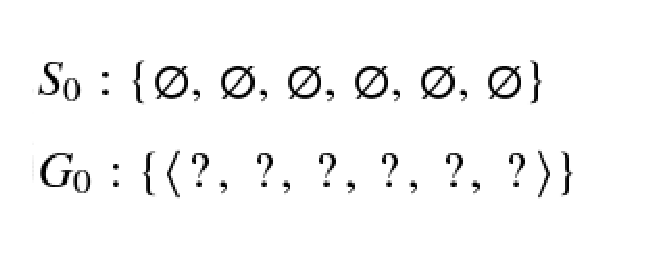
\includegraphics[scale=0.4]{exampleTrace.eps}
\end{figure}
\end{slide}


%%%%%%%%%%%%%%%%%%%%%%%%%%%%%%%%
\begin{slide}{Next Training Example and Classification?}
\begin{figure}
	\centering
	\includegraphics[scale=0.8]{../bookps/figure-vs3.ps}
\end{figure}
\small
\[ \langle Sunny\ Warm\ Normal\ Strong\ Cool\ Change \rangle \]
\[ \langle Rainy\ Cool\ Normal\ Light\ Warm\ Same \rangle \]
\[ \langle Sunny\ Warm\ Normal\ Light\ Warm\ Same \rangle \]

\end{slide}


%%%%%%%%%%%%%%%%%%%%%%%%%%%%%%%%
\begin{slide}{What Justifies this Inductive Leap?}
\[+\ \  \langle Sunny\ Warm\ Normal\ Strong\ Cool\ Change \rangle \]
\[+\ \  \langle Sunny\ Warm\ Normal\ Light\ Warm\ Same \rangle \]
\[S:\ \  \langle Sunny\ Warm\ Normal\ ?\ ?\ ? \rangle \]

Why believe we can classify the unseen
\[ \langle Sunny\ Warm\ Normal\ Strong\ Warm\ Same \rangle \]
\end{slide}


%%%%%%%%%%%%%%%%%%%%%%%%%%%%%%%%
\begin{slide}{An Unbiased Learner}
\begin{itemize}
	\item  Idea: Choose $H$ that expresses every teachable concept (i.e., $H$ is the power
set of $X$)
\item Consider $H' =$ disjunctions, conjunctions, negations over previous $H$.
\item For example \[  \langle Sunny\ Warm\ Normal\ ?\ ?\ ? \rangle  \vee  \neg \langle ?\ ?\ ?\ ?\ ?\ Change \rangle   \]
\item What are $S$, $G$ in this case?
\end{itemize}
\end{slide}


%%%%%%%%%%%%%%%%%%%%%%%%%%%%%%%%
\begin{slide}{Inductive Bias}
\small
\begin{itemize}
	\item Concept learning algorithm $L$ 
	\item Instances $X$, target concept $c$
	\item Training examples  $D_c = \{\langle x, c(x) \rangle \}$
	\item Let $L(x_i,D_c)$ denote the classification assigned to the instance $x_i$ by $L$ after training on data $D_c$.
\end{itemize}

{\bf Definition}:  
\begin{quote}The {\bf inductive bias}
of $L$ is any minimal set of assertions $B$ such that for any target concept
$c$ and corresponding training examples $D_c$
\end{quote}

\[
(\forall x_i \in X) [(B \wedge D_c \wedge x_i) \models L(x_i,D_c)]
\]
where $A \models B$ means $A$ logically entails $B$
\end{slide}


%%%%%%%%%%%%%%%%%%%%%%%%%%%%%%%%
\begin{slide}{Inductive Systems \& Equivalent Deductive Systems}
\begin{figure}
	\centering
	\includegraphics[scale=0.6]{../bookps/figure-vs-bias-new.ps}
\end{figure}
\end{slide}

%%%%%%%%%%%%%%%%%%%%%%%%%%%%%%%%
\begin{slide}{Three Learners with Different Biases}
\begin{itemize}
\item Rote learner: Store examples, Classify $x$ iff it matches previously
observed example.
\item Version space candidate elimination algorithm
\item Find-S
\end{itemize}
\end{slide}


%%%%%%%%%%%%%%%%%%%%%%%%%%%%%%%%
\begin{slide}{Review}
\begin{itemize}
\item Concept learning as search through $H$
\item General-to-specific ordering over $H$
\item Version space candidate elimination algorithm
\item $S$ and $G$ boundaries characterize learner's uncertainty
\item Learner can generate useful queries
\item Inductive leaps possible only if learner is biased
\item Inductive learners can be modelled by equivalent deductive systems
\end{itemize}
\end{slide}





\end{document}
